\documentclass[12pt,conference]{IEEEtran}
\IEEEoverridecommandlockouts
% The preceding line is only needed to identify funding in the first footnote. If that is unneeded, please comment it out.
\usepackage{cite}
\usepackage{amsmath,amssymb,amsfonts}
\usepackage{algorithmic}
\usepackage{graphicx}
\usepackage[rightcaption]{sidecap}
\usepackage{hyperref}
\usepackage{array}
\usepackage{textcomp}
\usepackage{xcolor}
\hypersetup{
    colorlinks=true,
    linkcolor=black,
    filecolor=magenta,      
    urlcolor=blue,
}
\def\BibTeX{{\rm B\kern-.05em{\sc i\kern-.025em b}\kern-.08em
    T\kern-.1667em\lower.7ex\hbox{E}\kern-.125emX}}


\begin{document}

\title{Week 3 / Git Assignment} 

\author{\IEEEauthorblockN{Constance Hendrix}
\IEEEauthorblockA{\textit{CS 6000 - Fall 2020 - \today} \\
\textit{University of Colorado, Colorado Springs (UCCS)}}
}


\maketitle

% \section{Introduction}
Greetings.  My name is Constance Hendrix.  I go-by Constance.  I’m a wife, an electrical engineer, a 30-year Air Force veteran, and a current Engineering Security PhD student here at UCCS (see Canvas picture in Figure \ref{fig:me}). 
\begin{SCfigure}[0.5][h]
    \caption{Constance, about to be fed, while on a overdue retreat!}
    \centering
    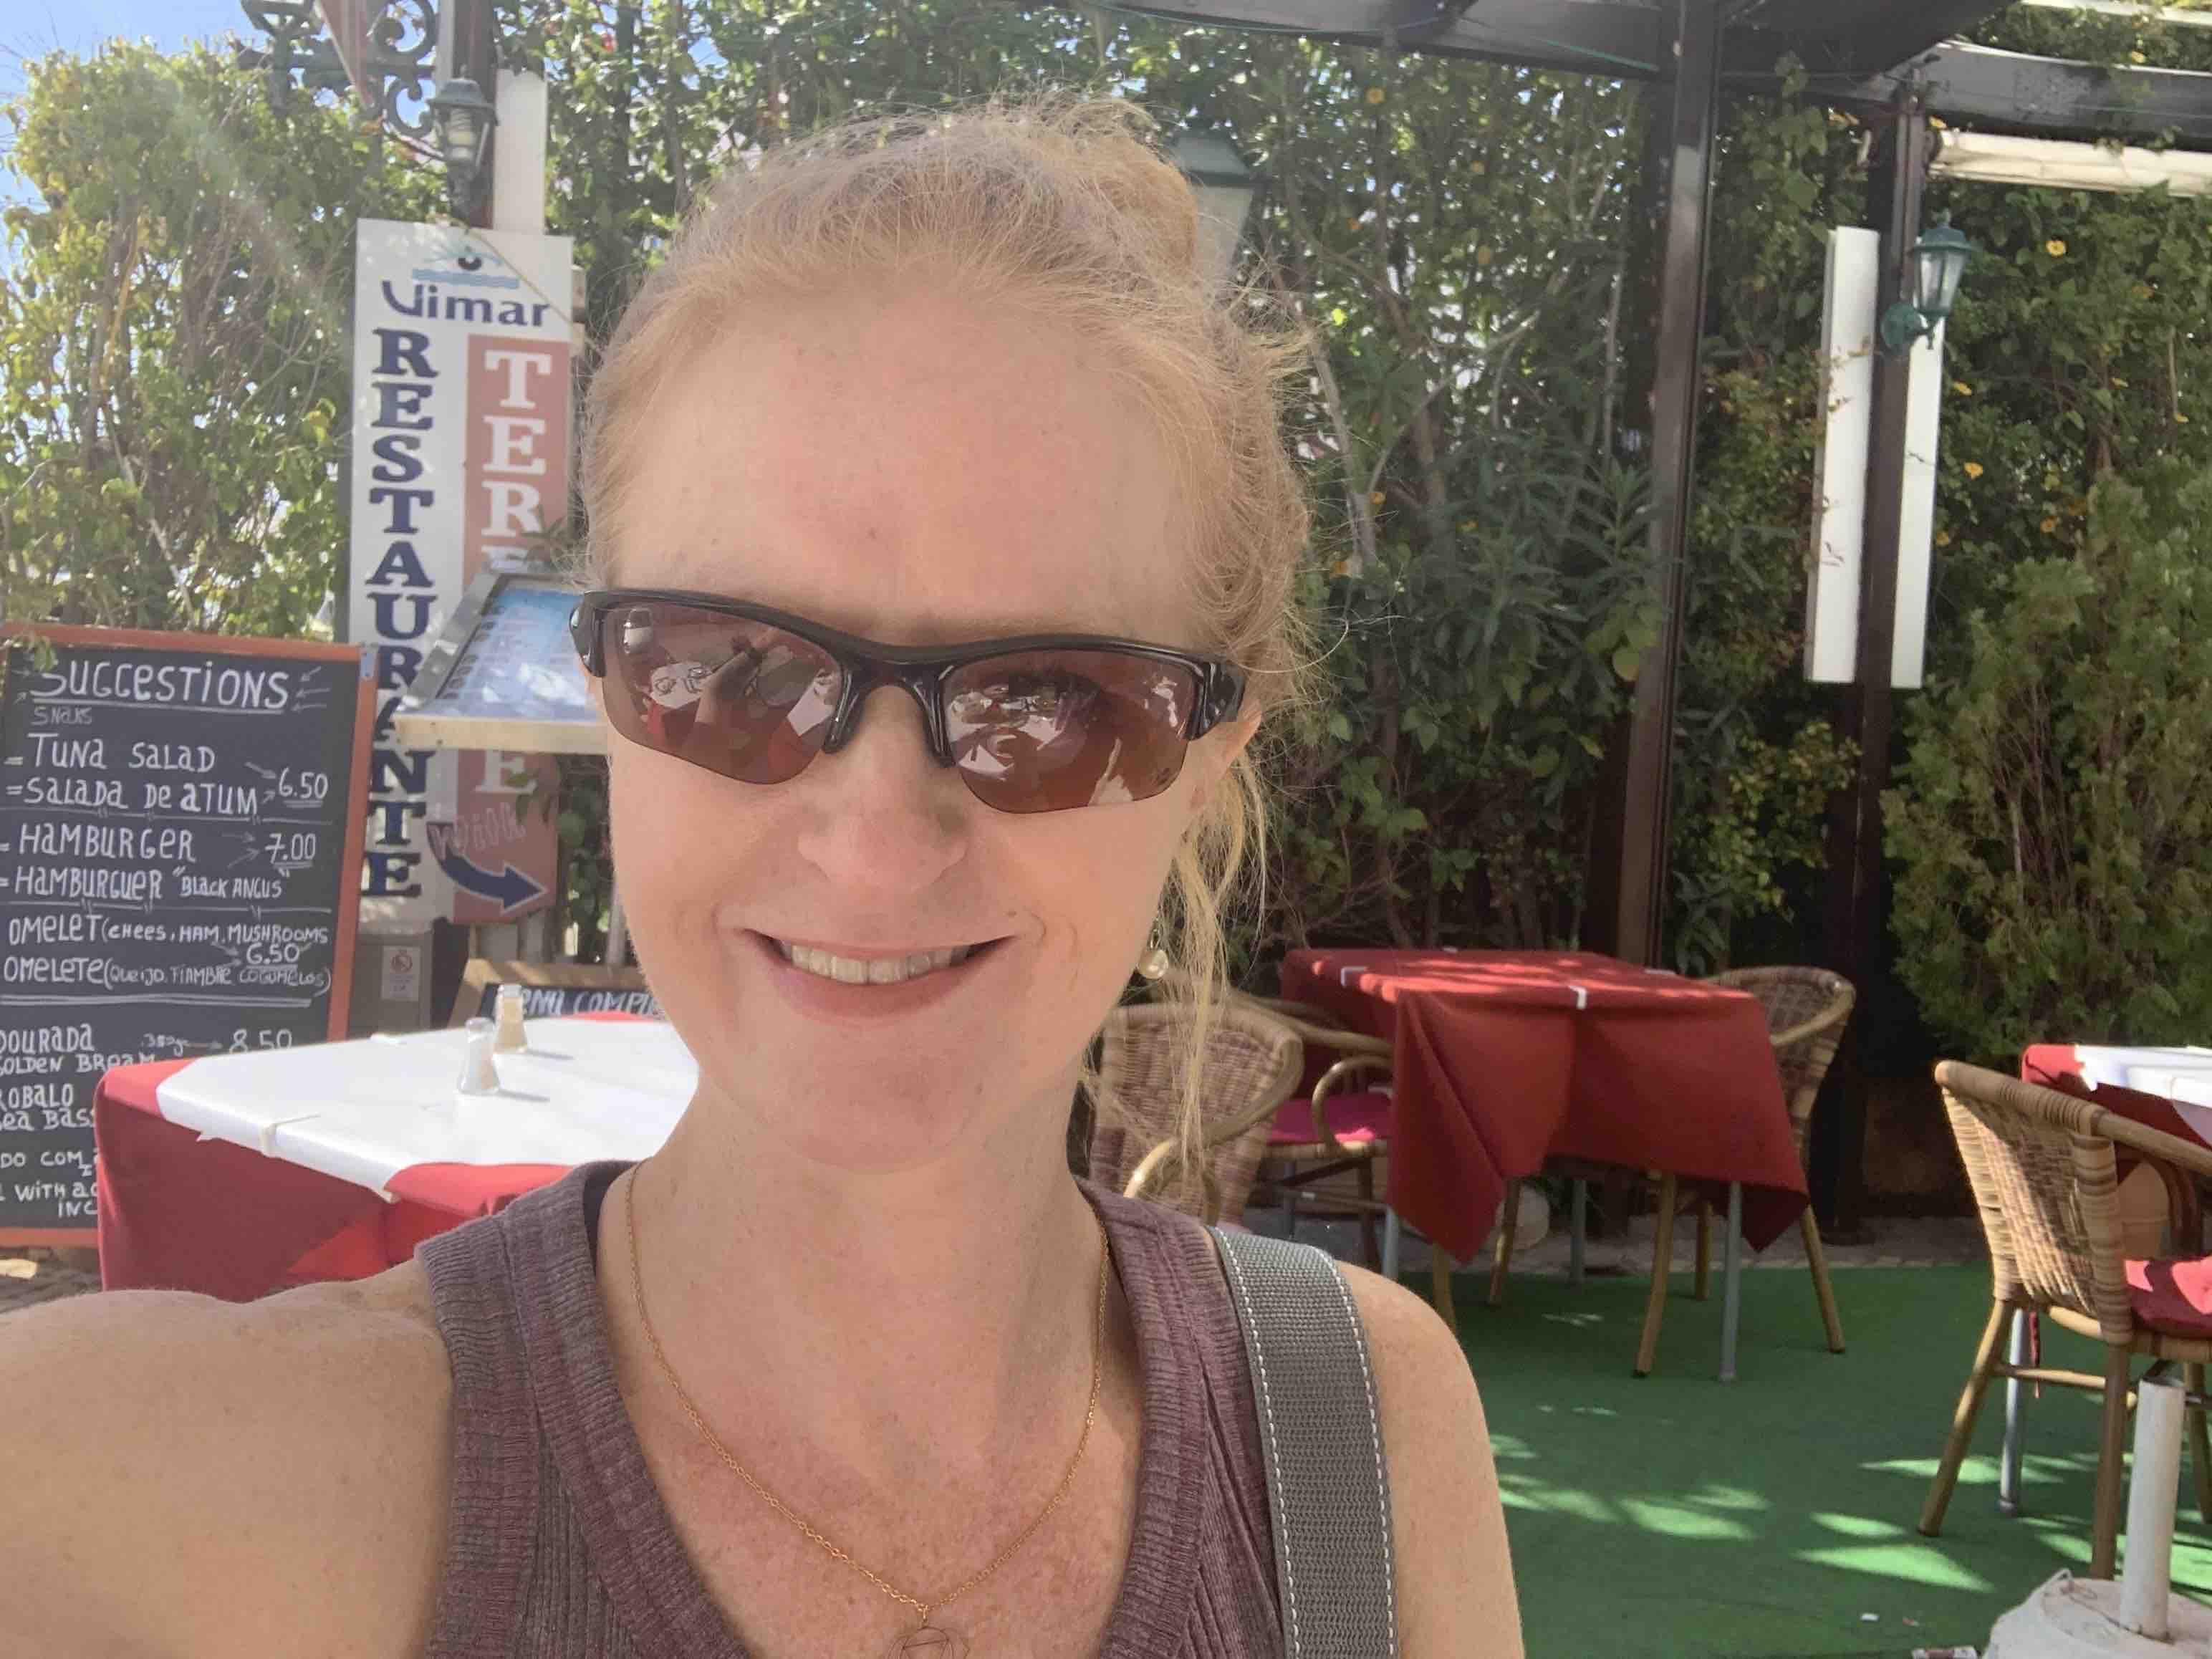
\includegraphics[scale=0.06]{canvas.jpg}
    \label{fig:me}
\end{SCfigure}
I’m coming in with a Masters of Science degree in electrical engineering with a focus in navigation systems from the Air Force Institute of Technology and a Masters of Business Administration from the University of West Florida.  I'm also a licensed electrical engineer in the state of Colorado and a certified Project Management Professional. My overarching goal for graduate school is to make a significant contribution to my engineering field and lay the foundation for a future in academia.  My research interests include reliable and accurate navigation, secure satellite communications, biologically-influenced design, artificial intelligence, and signal processing.  I have yet to specifically identify my security research topic, but know it will include artificial intelligence, signal processing, and//or edge computing. Over the Summer, I completed an Independent Study to narrow down my focus, but am having second thoughts about my selected research question and am currently investigating other options.  I hope to select a topic by next semester and will be preparing for my oral qualifier next Spring as well.  My goal for this course is to narrow my research focus for my degree, learn new and efficient ways to conduct research, and develop research questions. Outside of school, I work part-time as a position, navigation and timing (PNT) engineer, enjoy reading, working on stained glass creations, quilting, camping, fly fishing, hiking, cooking, and gardening.  Quilting is a tradition for the women in my family.  Last month, I completed my first quilt, which can be seen on my new and no-so-current blog at \url{constancehendrix.com}.  At my age, I am excited to finally carry on this tradition -- better late than never, I say!

\vspace{12pt}
\end{document}
